% =====================================================================
%  MEASURED RESULTS
%
%  Everything in this file comes from a generated table under
%  tables/generated/ or a generated figure under figures/generated/.
%  No value here was typed by hand. Each \input has a provenance header
%  naming the result file and the git commit it was produced from.
%
%  This file is kept separate from the synthetic body of main.tex on
%  purpose: while \synthdrafttrue is set, a reader must be able to tell
%  at a glance which numbers are real. Values here are wrapped in
%  \measured{} rather than \syn{}.
%
%  Regenerate with:  make aggregate figures tables
% =====================================================================

\section{Measured Results}
\label{sec:measured}

This section reports measurements taken on the radio-telemetry layer of
\DA{} under the run-disjoint protocol of Section~\ref{sec:setup}. Unless
stated otherwise every figure is a mean over \measured{20} split seeds,
with intervals given as paired $t$-intervals over split means. Model
seeds are nested inside split seeds and averaged before testing, so the
effective sample size is the number of splits, not the number of fits.

\subsection{Evaluation Protocol Effects}
\label{sec:measured:leakage}

We first quantify how much of a reported score is attributable to the
split protocol rather than to the detector. The same models, features and
seeds are evaluated twice: once under a random split over windows, the
convention in much of the intrusion-detection literature, and once under a
split in which whole capture runs are held out.

\begin{table}[t]
\caption{Effect of the split protocol on macro-$F_{1}$, \DA{} radio layer.
Differences are paired over \measured{20} split seeds; $^{\ast}$ marks
significance after Holm correction within the family of eight models.}
\label{tab:m_leakage}
\centering
% GENERATED by analysis/make_tables.py on 2026-09-20
% source: results\EXP-002\processed\leakage_summary.csv
% commit: 99f8635
% DO NOT EDIT. Edit the generator, re-run `make tables`.
mlp & 0.953 & 0.872 & +0.081 & [-0.008, +0.186] \\
rf & 0.970 & 0.871 & +0.099$^{\ast}$ & [+0.009, +0.204] \\
hgb & 0.983 & 0.870 & +0.113$^{\ast}$ & [+0.027, +0.209] \\
xgboost & 0.976 & 0.859 & +0.117$^{\ast}$ & [+0.029, +0.221] \\
tree & 0.956 & 0.822 & +0.134$^{\ast}$ & [+0.048, +0.226] \\
logreg & 0.835 & 0.802 & +0.034 & [-0.060, +0.127] \\
stratified & 0.499 & 0.508 & -0.009$^{\ast}$ & [-0.011, -0.006] \\
majority & 0.434 & 0.431 & +0.002 & [-0.009, +0.013] \\

\end{table}

Table~\ref{tab:m_leakage} and Fig.~\ref{fig:m_leakage} show the result. Every
non-trivial architecture scores materially higher under the random split,
and all six differences survive Holm correction. The effect is not small:
it ranges from \measured{9.3} to \measured{16.8} points of macro-$F_{1}$,
with paired effect sizes $d_{z}$ between \measured{0.78} and
\measured{1.35}.

Two features of the pattern matter more than its magnitude. First, the
ordering tracks model flexibility. A single depth-12 decision tree gains
most, the boosted ensembles next, the random forest and the multilayer
perceptron less, and logistic regression least. Second, the two trivial
baselines gain nothing: the majority-class classifier shows
$\Delta=\measured{-0.002}$ with $p=\measured{0.40}$. A classifier with no
capacity to memorise cannot profit from a leaky split, which is what
identifies the mechanism as memorisation rather than as a change in task
difficulty.

The practical consequence is that the inflation cannot be treated as a
constant offset. It is largest for precisely the flexible architectures
that are most often reported, so a reader cannot mentally discount a
published random-split figure by a fixed amount.

\begin{figure}[t]
\centering
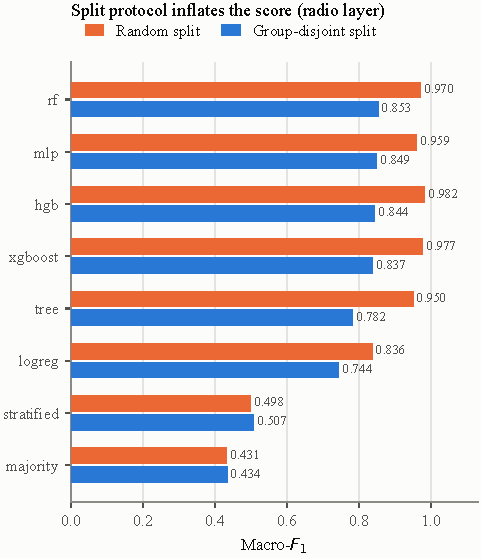
\includegraphics[width=\columnwidth]{../figures/generated/fig_leakage_radio.pdf}
\caption{Macro-$F_{1}$ under a random split and a run-disjoint split.
Bars are means over \measured{20} split seeds.}
\label{fig:m_leakage}
\end{figure}

\subsection{Operational Alert Burden}
\label{sec:measured:alerts}

Criterion 2 asks what the detector costs an operator rather than how it
scores on a corpus. Table~\ref{tab:m_alerts} reports both quantities side by
side at the default threshold, under the declared deployment parameters
$\pi=0.002$ and $\lambda_{b}=240{,}000$ benign flows per hour.

\begin{table}[t]
\caption{Corpus precision against operational precision, \DA{} radio
layer, $\tau=0.5$. Both $\pi$ and $\lambda_{b}$ are declared deployment
parameters, not measurements; Fig.~\ref{fig:m_alerts} sweeps them.}
\label{tab:m_alerts}
\centering
% GENERATED by analysis/make_tables.py on 2026-09-20
% source: results\EXP-004\processed\alert_burden_radio.csv
% commit: 1da178d
% DO NOT EDIT. Edit the generator, re-run `make tables`.
rf & 0.852 & 0.926 & 0.954 & 0.2619 & 63\,306 & 0.0814 \\
mlp & 0.847 & 0.933 & 0.937 & 0.2338 & 56\,571 & 0.0363 \\
hgb & 0.844 & 0.928 & 0.945 & 0.2569 & 62\,114 & 0.1291 \\
xgboost & 0.838 & 0.930 & 0.931 & 0.2467 & 59\,663 & 0.2185 \\
logreg & 0.744 & 0.930 & 0.798 & 0.2177 & 52\,638 & 0.0815 \\
majority & 0.434 & 0.766 & 1.000 & 1.0000 & 240\,481 & 0.0020 \\

\end{table}

The two precision columns are the criterion in one line. Corpus precision
sits between \measured{0.926} and \measured{0.933} for all five detectors,
a spread of \measured{0.007}. Once a realistic base rate is applied, the
operational precision of the same five spans \measured{0.036} to
\measured{0.218}, a factor of six. The metric a paper would report cannot
distinguish these detectors; the metric an operator lives with separates
them sharply. Absolute volumes are \measured{53{,}000} to
\measured{63{,}000} alerts per hour, the large majority of them false.

None of this is a new statistical result. The base-rate argument is
Axelsson's, and it is a quarter of a century old. What is new is its
quantification for a specific detector under a protocol that holds capture
runs out, reported alongside the tail-latency measurement for the same
model artefacts.

A second and less expected finding concerns the operator's only runtime
control. Sweeping the decision threshold to recover precision,
Table~\ref{tab:m_ppvcross} shows that $\text{PPV}=0.5$ is
\emph{unreachable at any threshold} for four of the five detectors. The
scores of the boosted models and the perceptron saturate near unity under
a run-disjoint split, so raising $\tau$ barely moves the alert volume: the
histogram-boosted ensemble still emits \measured{53{,}632} alerts per hour
at $\tau=\measured{0.99}$. Only the random forest and the linear model
reach $\text{PPV}=0.5$, and both do so by collapsing recall, to
\measured{0.418} and \measured{0.189} respectively. This is a calibration
failure with an immediate operational consequence, and it is invisible in
accuracy, $F_{1}$ or AUC.

\begin{table}[t]
\caption{Decision threshold required to reach a usable operational
precision, and its cost in recall and alert volume.}
\label{tab:m_ppvcross}
\centering
% GENERATED by analysis/make_tables.py on 2026-09-21
% source: results\EXP-004\processed\ppv_crossings_radio.csv
% commit: e45aa5b
% DO NOT EDIT. Edit the generator, then re-run `make tables`.
\begin{tabular}{lcccc}
\toprule
Model & PPV target & $\tau$ required & Recall & Alerts/h \\
\midrule
rf & 0.10 & 0.55 & 0.945 & 60\,768 \\
rf & 0.25 & 0.65 & 0.921 & 57\,251 \\
rf & 0.50 & 0.95 & 0.418 & 7\,521 \\
mlp & 0.10 & 0.60 & 0.922 & 52\,993 \\
mlp & 0.25 & 0.85 & 0.852 & 44\,500 \\
mlp & 0.50 & \textit{unreachable} & -- & -- \\
hgb & 0.10 & 0.40 & 0.948 & 62\,706 \\
hgb & 0.25 & 0.99 & 0.898 & 53\,632 \\
hgb & 0.50 & \textit{unreachable} & -- & -- \\
xgboost & 0.10 & 0.20 & 0.957 & 65\,758 \\
xgboost & 0.25 & 0.55 & 0.926 & 59\,036 \\
xgboost & 0.50 & \textit{unreachable} & -- & -- \\
logreg & 0.10 & 0.65 & 0.715 & 43\,305 \\
logreg & 0.25 & 0.85 & 0.514 & 26\,981 \\
logreg & 0.50 & 0.99 & 0.189 & 8\,855 \\
majority & 0.10 & \textit{unreachable} & -- & -- \\
majority & 0.25 & \textit{unreachable} & -- & -- \\
majority & 0.50 & \textit{unreachable} & -- & -- \\
\bottomrule
\end{tabular}

\end{table}

\begin{figure*}[t]
\centering
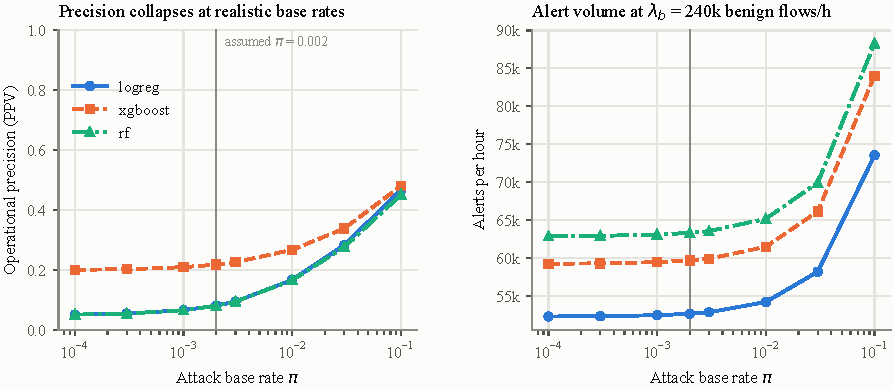
\includegraphics[width=\textwidth]{../figures/generated/fig_alert_burden.pdf}
\caption{Operational precision and alert volume against the attack base
rate $\pi$. Both panels share one vertical scale each; the vertical rule
marks the $\pi$ assumed in Table~\ref{tab:m_alerts}.}
\label{fig:m_alerts}
\end{figure*}

\subsection{Decision Latency Against a Swept Budget}
\label{sec:measured:latency}

\begin{table}[t]
\caption{Per-decision latency, \DA{} radio layer, \measured{1500}
repetitions after warm-up. The last column gives the smallest near-real-time
budget each architecture's 99th percentile conforms to.
\textbf{These are emulated measurements}; see Section~\ref{sec:limitations}.}
\label{tab:m_latency}
\centering
% GENERATED by analysis/make_tables.py on 2026-09-20
% source: results\EXP-005\processed\budget_sweep_radio.csv
% commit: 99f8635
% DO NOT EDIT. Edit the generator, re-run `make tables`.
FLOOR (no-op) & 0.01 & 0.02 & 0.10 & 0.53 & 1 \\
tree & 1.81 & 3.51 & 4.76 & 6.09 & 5 \\
logreg & 2.45 & 4.40 & 6.51 & 13.43 & 10 \\
xgboost & 3.83 & 6.19 & 7.29 & 11.39 & 10 \\
mlp & 2.25 & 4.95 & 8.17 & 13.98 & 10 \\
hgb & 53.16 & 74.76 & 94.62 & 446.06 & 100 \\
rf & 93.41 & 124.55 & 378.05 & 1034.91 & 500 \\

\end{table}

O-RAN specifies the near-real-time control loop over a range of 10\,ms to
1\,s rather than at a single value. Reporting conformance against one
chosen point inside that range makes the verdict an artefact of the
choice. Table~\ref{tab:m_latency} and Fig.~\ref{fig:m_latency} therefore report,
for each architecture, the smallest budget its 99th percentile conforms to.

The floor experiment was run first. A no-op model on the same path yields
$p_{99}=\measured{0.103}$\,ms, two orders of magnitude below the tightest
budget considered, so the ordering below is a property of the models rather
than of the measurement platform.

The verdict moves with the budget. At \measured{1}\,ms no architecture
conforms. At \measured{5}\,ms only the single decision tree does. At
\measured{10}\,ms four of six conform. At \measured{1000}\,ms all of them
do. One set of measurements thus supports four different conclusions,
separated only by where the line is drawn, which is the reason to report
the crossing point instead of a pass-fail column.

\begin{figure}[t]
\centering
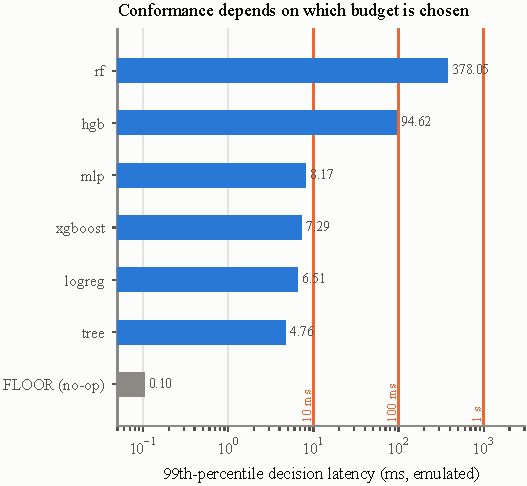
\includegraphics[width=\columnwidth]{../figures/generated/fig_latency_budget.pdf}
\caption{99th-percentile decision latency per architecture. Vertical rules
mark three points inside the specified near-real-time range.}
\label{fig:m_latency}
\end{figure}

Decomposing the path shows where the time goes. Model inference accounts
for \measured{0.18} to \measured{0.96}\,ms for the four architectures that
conform at 10\,ms, whereas constructing features from packets costs a
median \measured{6.90}\,ms per flow, ranging from \measured{4.49} to
\measured{37.34}\,ms across captures. For those architectures feature
construction is between \measured{7} and \measured{39} times the cost of
inference. The relation inverts for the random forest and the
histogram-boosted ensemble, whose own inference exceeds extraction, so the
observation is architecture-dependent and is stated as such.

Two caveats bound this. The exporter is a reference implementation in
Python running at \measured{1.1} to \measured{4.3}\,MB/s, and a native
implementation would be substantially faster; the defensible claim is
therefore that feature construction is of the same order as or larger than
inference for every architecture that meets a 10\,ms budget, so optimising
the model alone addresses the smaller part of the budget. Per-flow cost
also varies roughly eightfold across captures because it is driven by
packets per flow rather than by flow count, which is why the range is
reported beside the median.
